% This template has been downloaded from:
% http://www.LaTeXTemplates.com



%----------------------------------------------------------------------------------------
%	PACKAGES AND OTHER DOCUMENT CONFIGURATIONS
%----------------------------------------------------------------------------------------

\documentclass[oneside]{article}
\usepackage{multicol}



\usepackage{lipsum} % Package to generate dummy text throughout this template


\usepackage[T1]{fontenc} % Use 8-bit encoding that has 256 glyphs


\usepackage[hmarginratio=1:1,top=32mm,columnsep=20pt]{geometry} % Document margins
%\usepackage{multicol} % Used for the two-column layout of the document
\usepackage[hang, small,labelfont=bf,up,textfont=it,up]{caption} % Custom captions under/above floats in tables or figures
\usepackage{booktabs} % Horizontal rules in tables
\usepackage{float} % Required for tables and figures in the multi-column environment - they need to be placed in specific locations with the [H] (e.g. \begin{table}[H])
\usepackage{hyperref} % For hyperlinks in the PDF
\usepackage{listings}
\usepackage{url}
\usepackage{graphicx}
\usepackage{wrapfig}
\usepackage{caption}
%\graphicspath{ {image/} }

\usepackage{lettrine} % The lettrine is the first enlar ed letter at the beginning of the text
\usepackage{paralist} % Used for the compactitem environment which makes bullet points with less space between them

%\usepackage{abstract} % Allows abstract customization
%\renewcommand{\abstractnamefont}{\normalfont\bfseries} % Set the "Abstract" text to bold
%\renewcommand{\abstracttextfont}{\normalfont\small\itshape} % Set the abstract itself to small italic text


\usepackage{titlesec} % Allows customization of titles
\renewcommand\thesection{\arabic{section}} % Arabic numerals for the sections
\renewcommand\thesubsection{\arabic{section}.\arabic{subsection}} % Arabic numerals for subsections
\titleformat{\section}[block]{\large\scshape\centering}{\thesection}{1em}{} % Change the look of the section titles
\titleformat{\subsection}[block]{\large}{\thesubsection}{1em}{} % Change the look of the section titles

\usepackage{fancyhdr} % Headers and footers
\pagestyle{fancy} % All pages have headers and footers
\fancyhead{} % Blank out the default header
\fancyfoot{} % Blank out the default footer
%\fancyhead[C]{Running title $\bullet$ November 2012 $\bullet$ Vol. XXI, No. 1} % Custom header text
\fancyfoot[RO,LE]{\thepage} % Custom footer text

%----------------------------------------------------------------------------------------
%	TITLE SECTION
%----------------------------------------------------------------------------------------

\title{\vspace{-20mm}\fontsize{20pt}{10pt}\selectfont\textbf{Stuck in Traffic Final Project Report}}
\author{
\large
{Antria Dimitriou, Filippo Mariani, Maximilian Nikolaidis, Filippos Raditsas, Maxim Vasilishin}\\[10mm] % Your name
\normalsize King's College London \\ [50mm] % Your institution
\normalsize {\textit{7CCSMGPR Group Project: Traffic Management Simulation}}
%\normalsize \href{mailto:filippo.mariani@kcl.ac.uk}{filippo.mariani@kcl.ac.uk} % Your email address
\vspace{-85mm}
}
\date{}

%----------------------------------------------------------------------------------------

\begin{document}

\maketitle %add title

%\thispagestyle{fancy} % All pages have headers and footers

%----------------------------------------------------------------------------------------
%	ABSTRACT
%----------------------------------------------------------------------------------------

%\begin{abstract}

%\noindent \lipsum[0]  % Dummy abstract text

%\end{abstract}

%\clearpage 
%----------------------------------------------------------------------------------------
%	ARTICLE CONTENTS
%----------------------------------------------------------------------------------------

%\begin{multicols}{2} % Two-column layout throughout the main article text
\newpage

\section{Introduction}

Road traffic management is a well known problem in such big city like London. In the last few years a lot of research has been driven by the importance of improving traffic management in the best way possible. Our idea is to ultimately create a simulation platform that will be fully customizable by the users and will allow them to simulate the scenarios based on their preference. We will be using Java in Eclipse IDE as our main programming language and Photoshop for the creation of the graphics.
\newline

\noindent The aim of the report will be to produce a working traffic simulator, which is based on traffic management simulation software. Road traffic is a well-known problem in a big city like London, therefore the idea of this simulation is to create as near as possible traffic simulations as possible to avoid congestion and other road issues. The idea behind this simulation is to improve traffic management in the best possible way. Our project is to create a simulation platform that will be fully customizable by user and will allow them to simulate real life scenarios, as well as scenarios of their preference.
\newline

\noindent The programming language that will be used in the project is Java built in Eclipse IDE, the design program will be Photoshop.
The project will include the full development process relying upon UML diagrams in the analysis and design phases. The testing will be formalized and the user documentation will also be produced as part of the final submission. Every phase of this project will be presented in a report detailing the process clearly and its outcomes.
In this project there are four teams that each have several tasks to complete. These teams include an in depth analysis of the projects requirements, design and development, programming the software code, and finally quality assurance, testing and user documentation. 
\newline 

\noindent Our main aim and objectives for this traffic simulation is to provide a user with an intelligent traffic simulation engine easy to implement and customize in the future. Our main idea is to develop a road generator engine and an automatic path discovery system in order to allow new functionalities to be builded on top without affecting the main simulation engine.
\newline

\noindent Since we decided to use Java, we also had to think about the animation which requires repaint of the graphics so that the movement of the cars is smooth. To avoid performance issues and large memory consumption we will have to write a function which takes as a parameter the size and number contents of the grid and decides what the optimal repaint time threshold is. Additionally, in order to avoid implementing car to car communication algorithms and A.I, we decided to follow a predefined-path approach for the cars in the simulation. That way we allow the users to customize the simulation according to their needs instead of simulating a specific pseudorandom scenario that would be limited by the efficiency of our algorithms. Apart from that, we considered implementing more sophisticated methods infeasible for the timeframe given for this project. 
\newpage

\noindent The rest of the paper is organized as follow. Section 2 investigate some related traffic simulation project that help us understand define the requirement for our traffic simulation. Section 3 specify the requirement and an overview of the project description. Section 4 is the implementation chapter. In this chapter we will discuss in details our software simulator and what are the most important functionalities and how we accomplish that. Section 5 describe activity related to team work and how we used different tools and process to facilitate the collaboration during the project development. Section 6 present an overall project evaluation and propose some future work implementation. Ultimately in section 7 we will discuss about peer assessment and how we allocate points for our group members.

\section{Review: Describe related work}

The object of interest in this section is to review related developments and tools for traffic simulation systems. The main aim of this project is to simulate a dynamic software which controls the flow of the traffic by using the available development tools for its implementation. The related work is similar projects available in the industry which most of them are open-source software for multi-agents simulation for their development. Naturally, existing software will either outperform or lag regarding the objectives of our project. This kind of software may differ from other?s work in many aspects such as: 2-dimensional or 3-dimensional representation, quality of graphics, types of vehicles (cars, buses, taxis, long vehicles), traffic lights, types of roads (horizontal and vertical roads, intersection, single or double lane roads, roundabout, one-way road), external factors (parking slots, pedestrians, crossings), behavior of drivers (intelligence system), road works and much more. 
\newline

\noindent There are many open-source tools available in the market for developing simulation systems and traffic modeling; some them are Aimsun, TransModeler, RoadTrafficSimulator, AnyLogic, Sumo etc. Aimsun tool is one of the most famous integrated transports modeling software which intergrated by TSS. Many high-level projects have been developed with the help of Aimsun (reference website). 

\noindent In \cite{luke2005mason}we have identified is partially related with our project objective since it introduces multi-agent simulation toolkit developed using Java programming tool. The aim of this project is to make it easy to be modified both in programming and in graphical representation. 

\noindent In \cite{dotoli2006urban} the author introduces a modeling technique to describe the behavior of urban traffic systems by having as a case study a real intersection in a city of Italy, called Bari. The traffic network model has been generated by using the mathematical modeling language Petri Nets and the Coloured Timed Petri Net(CTPN) for describing the flow of vehicles. The idea behind this modeling technique is to show that a Petri Net model can be easily translated to traffic control simulation software with the appropriate programming skills but without any significant costs.
\newline

\noindent In \cite{tavladakis1999development} a system of intersection controllers in traffic lights is described. An area-wide traffic control system is presented by using predictions to test and control the functionality of the traffic lights in intersections. This system is considered as a cyclic system since the results taken from a current cycle (execution), and then they are used to test the behavior of the system for the next cycle. The system can only be used to control the traffic in isolated nodes as well as in the center of small towns but it cannot handle large and demanding roads.
\newline

\noindent In \cite{chinyere2011design} the authors introduces an intelligent system that has been built for monitoring and controlling the flow of traffic using Java programming language. They have used the methodology of Fuzzy Logic and the software was simulated and tested for a popular intersection in a Nigeria city to control the flow of the traffic. 
The objective of this paper matches with the objective of our project, where a dynamic software has been developed to be as efficient as well as user-friendly. 
\newline

\noindent In \cite{center1996intelligent} the project is based in fuzzy logic technology has been built to implement an intelligent traffic light controller in junctions developed in Visual Basic programming tool. It is also comparing fuzzy logic controller and a fixed-timer controller and the results of fuzzy controller tend to have better performance results during the simulation.
\newline

\noindent In \cite{sewall2010continuum} a well-developed model is presented and successfully handles lane changes and traffic behaviors based on different speed limits in order to have a scalable and interactive system for real-time scenarios. This method has been developed using the open-source traffic simulation package, SUMO, and it has been tested and proved that it can work on large, real-world road networks. 

\noindent In \cite{kareem2011intelligent} the paper focuses on three test cases of an intelligent traffic light system, which are empty street case, normal street case and crowded street case, which are proposed as an additional component for improving the traffic light configuration. 
\newpage

\section{Requirements and design: Project Description}

The aim of this project is to develop a simulation engine, which could be utilized for testing scenarios and potentially improve the well-known issue of traffic management and optimization. Our goal is to have abstract concepts that will allow us to simulate certain scenarios but also become an easy adaptive platform to build on top for future ideas. Our first level aim is to develop a platform which loads a map, identifies possible paths for the cars, supports two way vertical and horizontal roads, as well as intersections. The map has entry points and exit points; upon arrival to an exit point the car object will be deleted. Our initial model will have a car, which is going to follow all the possible paths of our sample map. The next step will be to add more cars onto the map, as well as traffic lights to control the traffic. If time allows it, we are planning to have multi-lane roads and support scenarios of different driving behaviors such as reckless driving, too slow driving and cases of "polite" drivers that give way to other cars in order to help the road's decongestion. Furthermore ideas for future implementation also include parking spots, emergency lanes and vehicles, as well as pedestrians crossing the road. 
\newline

\noindent For this group project we will implement and simulate some of the most common scenarios that can be experienced during a normal day. The simulation will present a scenario where two or more vehicles meet at an intersection and we will simulate how the traffic lights handle such scenarios to control traffic. The aim of the project is to have a first understanding of the problem faced by road traffic enforcement. The simulation will try to provide a solid starting block to further simulations and observations. For this reason users will be allowed to create their own maps. Upon initialization of our simulator and the choice of a map all possible paths are going to be calculated and all the cars entering the grid will have predefined randomly chosen starting and ending point as well as a path that they will follow. 

\noindent During the development of this project we have tried to set and satisfy some of the following requirements: 
\newline

\textbf {System requirements:}
\begin{itemize}
  \item System can identify possible paths for cars given a starting point and a final destination
  \item System supports different types of roads like: Horizontal block and vertical block, intersections, three input intersections, round-abound, horizontal and vertical double lane roads, double lane intersection, multi and single lane intersection
  \item System automatically detects intersection blocks and add traffic light 
  \item System will efficiently draw and evaluate road block in the simulation view (vertical, orizontal block, intersection, multi intersections)
  \item System will validate a map after user request 
  \item Vehicle Entrance \& Exit
  \item System set traffic simulation speed and numbers of cars???
  \item System resource consumption minimization (Java repaint picture)
 \end{itemize}
 
\textbf{User specifications:} 

\begin{itemize}
  \item Allow user to create and customize traffic map for simulation
  \item Allow user to load a predefined map from existing list
  \item Allow user to save, open, edit and delete new maps
  \item Allow user to check map validity 
  \item Allow user to time the simulation using the stopwatch functionalities
  \item Stopwatch functionalities allow user to start, stop, pause and refresh
  \item Allow user to easy navigate through menu bar section (Simulation, Map builder)
  \item Allow user to set traffic simulation speed and number of cars presented in the simulation ?
 	  	  
 \end{itemize}

\noindent  We have designed our simulation system in a way that when vehicles enter the simulation map the car already know the defined starting and end point of their journey. We thought this was the best scenario because allow us to simulate real life condition where driver already know their final destination. 
\newline

\textbf{In here we should present an high level UML diagram description}

\subsection{Methodology}

\noindent The Spiral model, has been used in order to keep up to date with completing the project. The spiral model is a risk driven process that allows all areas of the spiral to be created simultaneously in order for quick delivery. The spiral model is more appropriate for this kind of project, as it will help us mitigate risks such as steep learning curve during the development phase, limited time, and individual member's unforeseen circumstances and enable us to add features and ideas to the project. We have divided the spiral model in 4 main phases:

 \begin{itemize}
 \setlength\itemsep{-0.5em}
  \item Requirements Analysis: We investigated available open source libraries and formed our idea. 
  \item Risk Analysis: We will constantly evaluate the risk during the different phases of the project. 
  \item Development: After the initial risk analysis we start developing our project divided in tasks.
  \item Evaluation: We will maintain proper documentation and implementation requirements of each task. 	  	  
 \end{itemize}
 
 
%\begin{figure}[h]
%\centering
%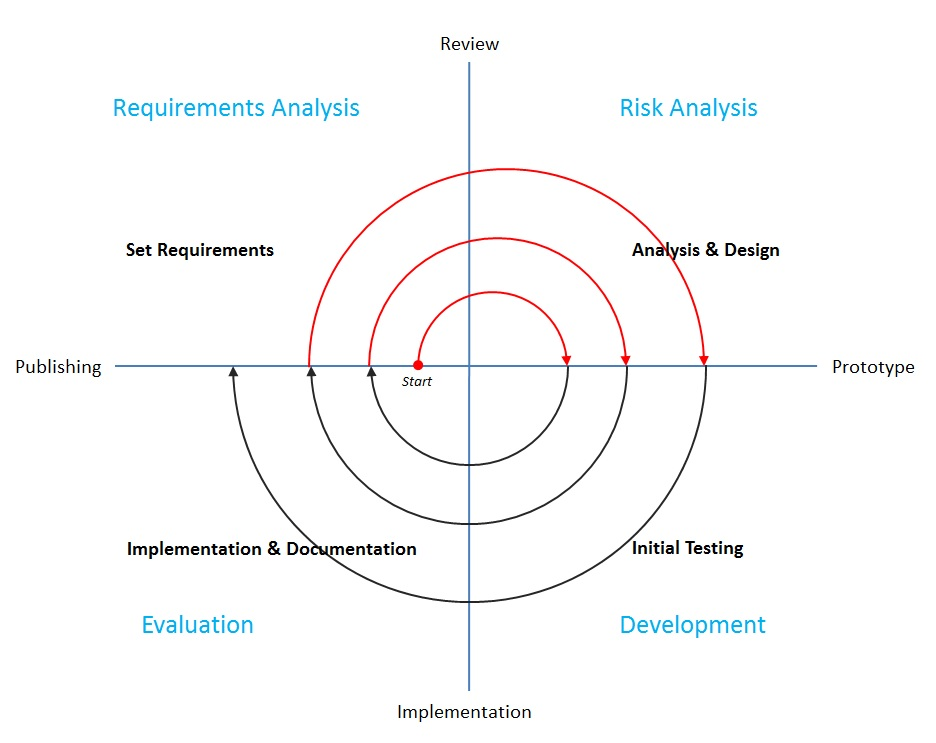
\includegraphics[width=4.5in]{spiralFINALv2}
%\caption{Spiral Model}
%\end{figure}
\newpage

\section{Implementation}

In this section we will describe the software implementation and details about the simulator view as well as core functionalities like road editor block, path discovery. We will then discuss problem we had during the implementation of this core functionalities and how we have tried to solve them in order to have a reliable system and traffic simulator. 
In this section we might want to present some source code snipped in each of the specific section. We have to be clear on how we implemented each and why we think it was a good idea.

\subsection{Road editor} Explain the main functionalities of it and how max implemented. Mainly deceive core function / variable 

\subsection{Path Discovery} Explain the main functionalities of it and how max implemented. Mainly deceive core function / variable 

\subsection{Simulation View} Explain the main functionalities of it and how max implemented. Mainly deceive core function / variable 

\subsection{Map validator for traffic simulation} Explain the main functionalities of it and how max implemented. Mainly deceive core function / variable 
\newpage


\section{Team Work}

Stuck in traffic will use the expertise of each member in each phase of the project in order to complete all required tasks. Our goal is to exchange knowledge and build not only a great traffic simulator but also develop teamwork skills. 
Our solution will provide users with a list of maps from which they can choose one to perform their simulation, as well as customize the number of cars and other parameters. In order to deliver this task we aim to provide users with good quality User Experience Design (UEX).

\noindent Even though all members will actively participate during all phase of the project development we have defied the lead of each phase which are included below.  

\begin{itemize} 

\item Project coordinator: Filippos Raditsas.
\item Analysis: Filippo Mariani.
\item Software Design/Development: Maxim Vasilishin.
\item Graphics: Maximimilian Nikolaidis.
\item GUI Design \& Development: Antria Dimitriou, Filippo Mariani.
\item QA: Antria Dimitriou.

\end{itemize}


\subsection{Analysis Team Responsibilities}

The analysis phase included the analysis of feasible technologies, programming languages, solutions, and approaches were evaluated to determine what route is best to take while continuing with the project. During this phase team members collaborated and brought their own thoughts and recommendations to the group to better determine all possibilities that the project could take. 
The analysis team is responsible for analyzing the specification given by the client and determining the conceptual model that will be used to structure the program around.



\subsection{Software Design \& Development Team Responsibilities}

This team is responsible for the high level design of the project assisting in the transition from requirements to technical specifications leading to the core development of the source code. The main software design and development team's responsibilities are to design the overall structure of the project following two essential parts; the higher level design and the detailed level design. 
\newline

\noindent In here we mainly have to mention maxim work and how first we/ he did an high-level analysis of the requirements and how we/he then translated in low level implementation.
\newline


\noindent One of the programming team\ 's tasks is to fully come to grips with the specification of the project. The lead developer team will discuss various aspects of the project as well as possible implementations with the whole team. 
The programming team\'s main responsibility falls upon working on the core source code development for the project. They will examine the high and low level designs and will transform them into functional Java code. 
Subsequently the programming team will be tasked with discovery and removing any errors or bugs presented in the final software.
Once the main project objectifies are completed (cars, roads, traffic lights) the programming team can then move onto the extra implemented features i.e.  car speed, parking lots, reckless driver, emergency vehicle ecc.


\subsection{The Graphics Team Responsibilities}

The graphics team was responsible for the creation of all the image and picture that will be used for our project. We decided to design everything from scratch trying to maintain avery  high level quality of the proposed images such as cars, intersections, traffic light, GUI button and graphics.
The graphics design team will work closely with the lead developers to produce an appropriate GUI that will be integrated in our platform in order to make the user experience more interactive and enjoyable. The design team will provide the graphics that are seen in the simulator, these include: cars, roads, intersections, stop lights, and any other graphic based structure

\subsection{QA Team Responsibilities}

The QA team or Test team's responsibilities is to test the deliverables of the project and to ensure all components gel and are consistent. At this point it is understood that the project will work to a modular design, with the possibility of running the development as waterfall. However the QA team will likely have scope to expand the project to an agile development should the need arise.
The QA team will be closely linked with the design and analysis teams to ensure the testing design is linked to the specification. A suitable testing framework will also be decided upon.
QA will perform testing of the simulator to ensure all components work smoothly are and consistent with the specifications and requirements. All the bugs found will be reported to the development team and if changes are necessary they will be handed over to the analysis team to perform a requirements analysis. The team will also be in charge of presenting and publishing the tests


\subsection{Team Management}

Effective and in time communication between partners was a key point for a proper project development. 
We have agreed to have a full group meeting every Wednesday at 17:00 in the MSc lab 543 to discuss any issue raised during the weekly task. There are also informal meeting that take place between the available members during the week, to discuss minor changes and alterations of the project. Informal meetings are not necessary for all members to attend these due to outside obligations such as: work, timetabling collusions from other lectures. Github was another valuable resources that helps us during the project to maintain a proper team work contribution in a very organized way. Our Github "Stuck In Traffic" repository can be accessed at the following link: https://github.com/philiprad/stuckintraffic. Github was used to upload development progress online and to allow members to maintain an up to date software development environment.


\noindent For internal communication that does not take place in person, the team have set up two mediums of communication; 

 \begin{itemize} 
  \item Slack Framework: https://slack.com/ We have created a group account to communicate and exchange files  
  \item Skype Conference: http://www.skype.com/en/ We have created an internal schedule for online meetings. 
 \end{itemize}
\newpage

\noindent In order to maintain a proper time management we have created and followed a gantt chart model. The chart has been used in order to set a proper structure for internal project deadline and to have a more accurate and reasonable workflow distribution among our group during the project time. We have divided the project in two different gant chart one for the intermediate project deadline and the second one for the final project deadline. 

\begin{figure}[h]
\centering
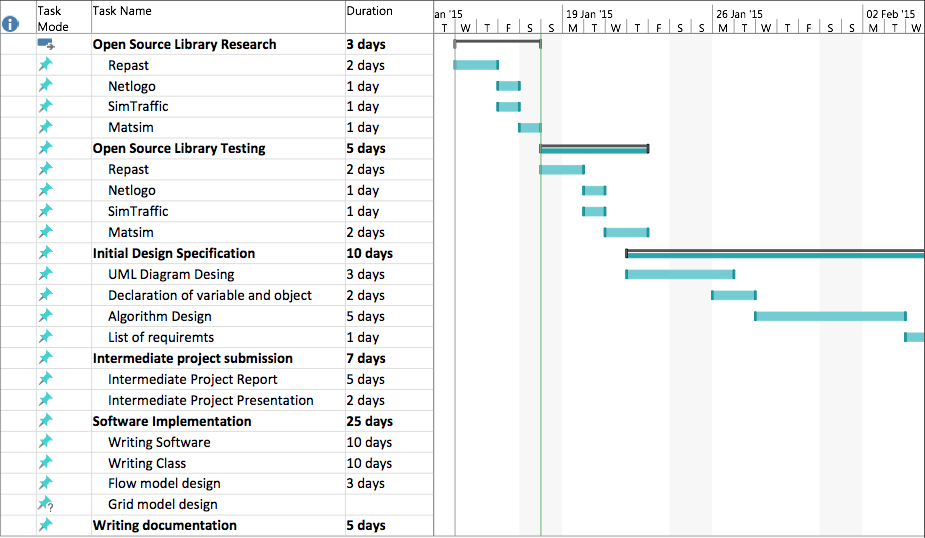
\includegraphics[width=6.5in]{ganttchart_old}
\caption{Gantt Chart depicting main tasks and timetable for intermediate report}
\end{figure}

\newpage
\begin{figure}[h2]
\centering
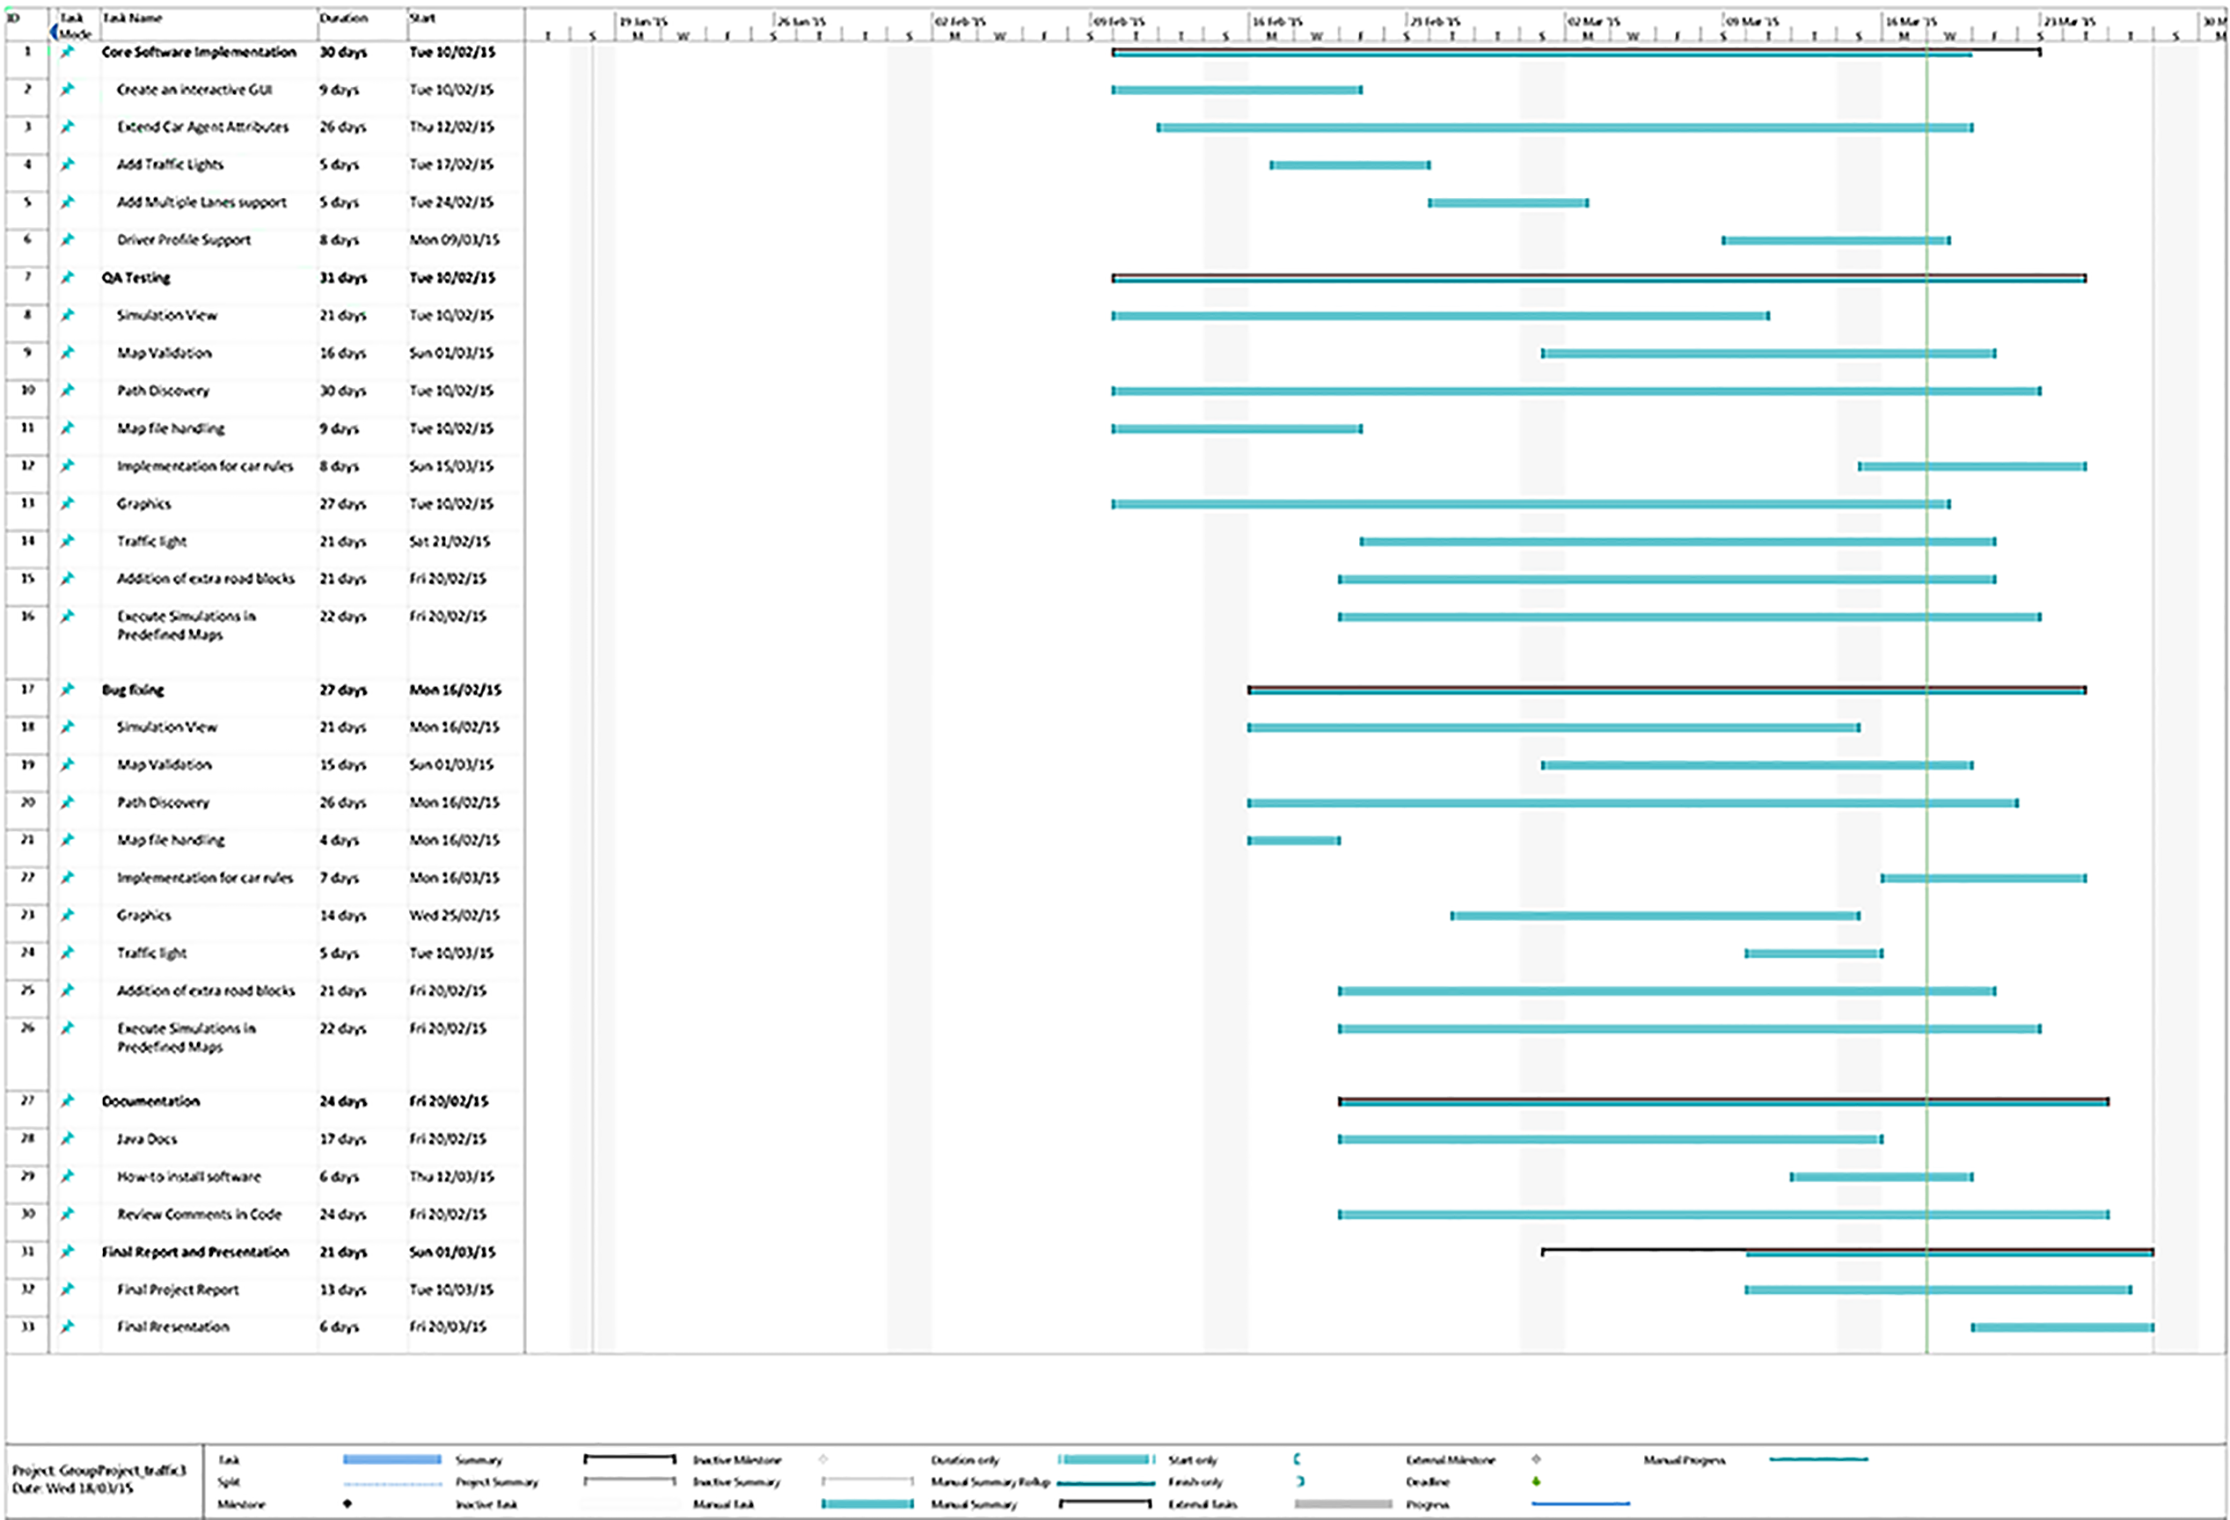
\includegraphics[width=6.5in]{GroupProject_traffic3_Final}
\caption{Gantt Chart depicting main tasks and timetable for final software and report submission}
\end{figure}
\newpage

\section{Project Evaluation}

\noindent Critically evaluate your project: what worked well, and what didn\ 't how did you do relative to your plan? what changes were the result of improved thinking and what changes were forced upon you? how did your team work together? etc. Note that you need to show that you understand the weaknesses in your work as well as its strengths. You may wish to identify relevant future work that could be done on your project.
\newline

\noindent During the project we have come across different problem and issue mainly related to the software implementation and during the design phase. The main problem we have at the beginning it was the big technical gap with our team leader developer. At the beginning we have to think on how to split each task properly given the knowledge of the people in the group. We were not all confident when using Github but this process help us to better split the work and specific contribution for different tasks. After experimenting with Github we have also created different brach in our master Github repository in order to keep working at the same time on different task without affecting the master branch file. For example the Filippo\_Andria brach (\url{https://github.com/philiprad/stuckintraffic/tree/Filippo_Andria}) has been created only for the GUI design and implementation. By doing this we allowed our lead developer to evaluate the proposed work and provide feedback for the proposed version of the GUI. 
\newline

\noindent Our project will possibly allow future developer to have a highly customized and reliable traffic simulation platform. We developed our system is a way that will easily allow developer and user to customize and improve our functionalities. Due to the project time limitation we were not able to implement all of the proposed functionalities such as: Different Driver Behavior, Parking spots, emergency lane support, pedestrians. This was mainly due to the fact that we have to allocate more time that initially thought for the roundabound implementation followed by a proper traffic light position allocator for all the given traffic intersections. After completing this task we have encounter some other problem mainly related to the map validation in the simulation view. Map validator function allow users to build and assemble road block given their specific requirement. During this phase we have to make a lot of test for the block validation in order to avoid validating non usable map. For this reason we have created a test script document called "Map Validation" that allow us to properly test the map validating process and add develop specific solution.
\newline

\noindent Given our current software structure and class division we believe that the above functionalities will be implemented easily in future version of the "Stuck in Traffic Simulator". Another important future work implementation is the aim of adding some statistical report generator about current traffic simulations such as allow the user to obtain information about number of cars, average car speed and potentially calculate the CO2 emission. Another future implementation we propose for our system is the support for emergency vehicle and how the traffic flow will change according with their presence. 
\newline

\noindent However not all the problem we had were related to technical issue. Another problem is that one of our group member was away for 10 days during the project. This was a problem for us because we have to split all the workload between the rest of us. For this reason we also decide to adopt the spiral model which allowed us to help each other during different project phase. (I don't know what bullshit to say for justify this)


\newpage
\section{Peer Assessment}

The following peer assessment plan ensures a fair distribution of merits upon completion of the project. It is vital that every member of "Stuck in Traffic" reads and fully understands the following text in regards to point allocation.
\newline

\noindent 
The peer assessment takes place to ensure a fair distribution of points for each member upon completion of the project. The amount of points awarded to a particular member may alter based on their contribution to the project and amount of work they put towards helping other members. Since there are five members in the team and there are 100 points to give accordingly the ultimate goal of our team is to evenly distribute the points assuming that we will all contribute the same amount of work and will collaborate smoothly and efficiently.
The points awarded to a particular member may alter based on their contribution to the project and amount of consideration towards other members. It is important to note that points can be deducted from a member as a penalty if their contribution towards the project has not been met or based on various negative actions. 
It has been taken into account for each members the participation in to the project, how much work has been submitted by each member, member\ 's enthusiasm and general involvement with the project activity.
\newline

\noindent Before the final deadline of this project, a final group meeting has been scheduled where members will fill out their personal peer assessment. Upon completion of the peer assessment members can openly discuss the point\'s award to them, if members feel that the amount of points awarded to them is unjust (In the event a member feels their total points are unfair and a compromise cannot be reached they shall be given an opportunity to explain to the team their reasons). The remaining members of the team shall then vote as to whether they feel the individuals mark is fair. If there is a unanimous decision among all other members then the individual must accept their amount of merit to be of a fair distribution. 
\newline

\noindent The peer assessment will be tallied positively or negatively on the determining criteria below:

 \begin{itemize} 
\item Failure to attend meetings where your presence has been required. Allowances can be made if the team agree the individual has a valid reason for their absence. In these circumstances it is vital that the team is informed with as much notice as possible.

\item Repeated failure to meet deadlines can also incur a penalty. It is possible that a deadline may have been too tight or other circumstances have made it unable to meet a deadline such as illness. In order to not face a penalty members are required to express any concerns about not meeting a deadline to the team during meetings. It shall be taken as a serious issue if a member fails to meet a deadline and becomes un-contactable.

\item The quality of your work may be taken into consideration. If a member feels the quality of another members work is inadequate they should inform them and the matter will be discussed in the next possible group meeting. The team will then discuss the work with the contributing member and find ways in which it can be improved. Penalties will only occur with repeated poor performance or an unreasonable unwillingness to improve work. 
 \end{itemize}
\newpage

\noindent The way in which a member will be allocated points is by the following table, each member will be able to give out one hundred (100) points in total. The points can range from 0 to 100 inclusive, also the members are able to assign decimal points to members, but the total amount of points must equal one hundred(100).
	
\begin{table}[h]
\resizebox{\textwidth}{!}{%
\begin{tabular}{|l|l|l|l|l|l|}
\hline
Name                  & Filippo Mariani & Maxim Vasilishin & Filippos Raditsas & Maximilian Nikolaides & Antria Dimitriou \\ \hline
Filippo Mariani       & 0               & 25               & 25                & 25                    & 25               \\ \hline
Maxim Vasilishin      & 25              & 0                & 25                & 25                    & 25               \\ \hline
Filippos Raditsas     & 25              & 25               & 0                 & 25                    & 25               \\ \hline
Maximilian Nikolaides & 25              & 25               & 25                & 0                     & 25               \\ \hline
Antria Dimitriou      & 25              & 25               & 25                & 25                    & 0                \\ \hline

\end{tabular}
}
\caption{Peer Assessment table}
\end{table}
%\clearpage

%\newpage
\section*{Source code software appendix} % Main appendix title

%\label{AppendixA} % For referencing this appendix elsewhere, use \ref{AppendixA}

Stuck in traffic source code: Simulation view % This is for the header on each page - perhaps a shortened title

\lstset{language=Java, framexleftmargin=0pt, framexrightmargin=10pt, frame=single, breaklines=true, }          % Set your language (you can change the language for each code-block optionally) 

\begin{lstlisting}[numbers=left, numberstyle=\small, numbersep=8pt,  framexleftmargin=1pt, framexrightmargin=10pt ]  % Start your code-block
/*
 * @author  Maxim Vasilishin
 * @version 1.0
 */
package gui;

import gui.RoadEditorView.ExitListener;
import gui.RoadEditorView.MainMenuListener;
//import gui.RoadEditorView.OpenListener;
import java.awt.BorderLayout;
import java.awt.Button;
import java.awt.Color;
import java.awt.Component;
import java.awt.Dimension;
import java.awt.EventQueue;
import java.awt.Font;
import java.awt.event.ActionEvent;
import java.awt.event.ActionListener;
import java.nio.Buffer;
import java.text.DecimalFormat;
import javax.swing.Box;
import javax.swing.ImageIcon;
import javax.swing.JButton;
import javax.swing.JFrame;
import javax.swing.JLabel;
import javax.swing.JMenu;
import javax.swing.Timer;
import javax.swing.JMenuBar;
import javax.swing.JMenuItem;
import javax.swing.JPanel;
import javax.swing.JScrollBar;
import javax.swing.JSeparator;
import javax.swing.JToolBar;
import javax.swing.SwingConstants;
import javax.swing.UIManager;
import javax.swing.UnsupportedLookAndFeelException;
import javax.swing.border.EmptyBorder;


// TODO: Auto-generated Javadoc
/**
 * The Class SimulationView.
 */
public class SimulationView extends JPanel{

	
    private JButton playButton;
	private JButton pauseButton;
	private JButton stopButton;	
	private JButton refreshButton;
	private JLabel displayTimer;

    private byte centiseconds = 0;
    private byte seconds = 0;
    private short minutes = 0;
    private DecimalFormat timeFormatter;//timer display format
    private Timer simulationTimer;
    
	
	/** The frame. */
	public ApplicationFrame frame;
	
	/**
	 * Instantiates a new simulation view.
	 *
	 * @param frame
	 *            the frame
	 */
	public SimulationView(ApplicationFrame frame){
		this.frame = frame;
		this.setLayout(new BorderLayout());
		JMenuBar menuBarTop = new JMenuBar();
		JMenu fileMenu = new JMenu("File");
	    menuBarTop.add(fileMenu);
	    JMenu editMenu = new JMenu("Edit");
	    menuBarTop.add(editMenu);
	    
	    frame.setJMenuBar(menuBarTop);
	    
	    JMenuItem newMap = new JMenuItem("New");
	    JMenuItem openMap = new JMenuItem("Open");
	    //openMap.addActionListener(new OpenListener());
	    JMenuItem exitMainMenu = new JMenuItem("Main Menu");
	    exitMainMenu.addActionListener(new MainMenuListener());
	    JMenuItem exit = new JMenuItem("Exit");
	    exit.addActionListener(new ExitListener());
        JMenuItem saveMap = new JMenuItem("Save");
        JMenuItem deleteMap = new JMenuItem("Delete");
        JMenuItem clearMap = new JMenuItem("Clear");
        fileMenu.add(newMap);
        fileMenu.add(openMap);
        fileMenu.addSeparator();
        fileMenu.add(exitMainMenu);
        fileMenu.add(exit);
        editMenu.add(saveMap);
        editMenu.add(clearMap);
        editMenu.add(deleteMap);
     
        //-----------------------------timer implementation
		JMenuBar menubar = new JMenuBar();
	    this.add(menubar, BorderLayout.NORTH);
	    
	    ImageIcon playImage = new ImageIcon("./images/play.png");
		ImageIcon stopImage = new ImageIcon("./images/stop.png");
		ImageIcon pauseImage = new ImageIcon("./images/pause.png");
		ImageIcon refreshImage = new ImageIcon("./images/refresh.jpg");
		
		playButton = new JButton(playImage);
		pauseButton = new JButton(pauseImage);
		stopButton = new JButton(stopImage);	
		refreshButton = new JButton(refreshImage);
		displayTimer = new JLabel("Display Timer");
	    JLabel timerLabel = new JLabel("Timer: ");
	   // simulationTimer = new Timer();
	    timeFormatter = new DecimalFormat("00");
	    
        
	playButton.addActionListener(new PlayListener());
	pauseButton.addActionListener(new PauseListener());
	stopButton.addActionListener(new StopListener());
	refreshButton.addActionListener(new RefreshListener());
	simulationTimer = new Timer(10, new ActionListener() {
         @Override
         public void actionPerformed(ActionEvent e) {
         	if(centiseconds<99){	
         		centiseconds++;
         	} else {
         		if(centiseconds==99){
         			seconds++;
         			centiseconds=0; 
         		}else if(seconds<60){
         				seconds++;
         			} else {
         				if(seconds==60){
         				minutes++;
         				seconds=0;
         			}
         		}
         	}
             displayTimer.setText(timeFormatter.format(minutes) + ":"
                     + timeFormatter.format(seconds) + "."
                     + timeFormatter.format(centiseconds));
         }
     });

	displayTimer.setText(timeFormatter.format(minutes) + ":"
             + timeFormatter.format(seconds) + "."
             + timeFormatter.format(centiseconds));

	
		
		//space between buttons
		menubar.add(timerLabel);
		menubar.add(Box.createRigidArea(new Dimension(10,0)));
		menubar.add(displayTimer);
		menubar.add(Box.createRigidArea(new Dimension(20,0)));
		menubar.add(playButton);
		menubar.add(Box.createRigidArea(new Dimension(10,0)));
		menubar.add(pauseButton); 
		menubar.add(Box.createRigidArea(new Dimension(10,0)));
		menubar.add(stopButton);
		menubar.add(Box.createRigidArea(new Dimension(10,0)));
		menubar.add(refreshButton);  
		
		
	
		/*JButton mainMenu = new JButton("Main Menu");
		mainMenu.addActionListener(new MainMenuListener());
		menubar.add(mainMenu);*/
		
		JToolBar toolbar = new JToolBar(JToolBar.VERTICAL);
		toolbar.setFloatable(false);
		this.add(toolbar, BorderLayout.EAST);
		
		JButton selectMapButton = new JButton("Open Sets of Maps");
		//selectMapButton.addActionListener(new OpenListener());
		selectMapButton.setAlignmentX(Component.CENTER_ALIGNMENT);
		toolbar.add(selectMapButton);
		//selectMapButton.setBackground(new Color(100,100,204));
		Font font = new Font("Avenir Book", Font.BOLD, 14);
		selectMapButton.setFont(font);
		selectMapButton.setForeground(Color.BLUE);
		toolbar.setPreferredSize(new Dimension(200,200));
		toolbar.add(selectMapButton);
		toolbar.addSeparator(new Dimension(100,150));
		
		JLabel carLabel= new JLabel("Select Number of Cars");
		carLabel.setFont(font);
		carLabel.setAlignmentX(Component.CENTER_ALIGNMENT);
		toolbar.add(carLabel);
		
		// 0 to n. n will be automatically calculated
		//TODO SET TO MAX
		JScrollBar carScrollBar = new JScrollBar(JScrollBar.HORIZONTAL, 1, 10, 0, 100); 
		carScrollBar.setAlignmentY(Component.TOP_ALIGNMENT);
		carScrollBar.setMinimum(1);
		carScrollBar.setMaximum(100);
		JLabel limitsLabel = new JLabel();
		limitsLabel.setText("" +carScrollBar.getMinimum() + "                              " + carScrollBar.getMaximum());
		limitsLabel.setAlignmentX(Component.CENTER_ALIGNMENT);
		toolbar.setPreferredSize(new Dimension(200,200));
		toolbar.add(carScrollBar);
		toolbar.add(limitsLabel);
		toolbar.addSeparator(new Dimension(100,150));
	
		
		JLabel motionLabel= new JLabel("Select Car Speed"); 
		motionLabel.setFont(font);
		motionLabel.setAlignmentX(Component.CENTER_ALIGNMENT);
		
		toolbar.add(motionLabel);
		JScrollBar motionScrollBar = new JScrollBar(JScrollBar.HORIZONTAL,1, 1, 0, 10);
		motionScrollBar.setAlignmentY(Component.TOP_ALIGNMENT);
		motionScrollBar.setMinimum(1);
		motionScrollBar.setMaximum(10);
		JLabel mLabel = new JLabel();
		mLabel.setText("" +motionScrollBar.getMinimum() + "                               " + motionScrollBar.getMaximum());
		mLabel.setAlignmentX(Component.CENTER_ALIGNMENT);
		
		toolbar.setPreferredSize(new Dimension(200,200));
		toolbar.add(motionScrollBar);
		toolbar.add(mLabel);
		toolbar.addSeparator(new Dimension(100,150)); //(new JSeparator(SwingConstants.HORIZONTAL));

	}
	
	
	
	/**
	 * The listener interface for receiving mainMenu events. The class that is
	 * interested in processing a mainMenu event implements this interface, and
	 * the object created with that class is registered with a component using
	 * the component's <code>addMainMenuListener<code> method. When
	 * the mainMenu event occurs, that object's appropriate
	 * method is invoked.
	 *
	 * @see MainMenuEvent
	 */

	
	public class MainMenuListener implements ActionListener{
		
		/* (non-Javadoc)
		 * @see java.awt.event.ActionListener#actionPerformed(java.awt.event.ActionEvent)
		 */
		public void actionPerformed(ActionEvent arg0){
			frame.removeView();
			frame.addView(new MainView(frame));
		}
	}
	
	//listener for exit
	public class ExitListener implements ActionListener{	
		/* (non-Javadoc)
		 * @see java.awt.event.ActionListener#actionPerformed(java.awt.event.ActionEvent)
		 */
		public void actionPerformed(ActionEvent arg0){
			System.exit(0);
		}
	}
	
	
	/*public class OpenListener implements ActionListener{
		public void actionPerformed(ActionEvent arg0){
			MapChoiceView openMap = new MapChoiceView();
		}
	}
	
	public class MapListener implements ActionListener{
		public void actionPerformed(ActionEvent arg0){
			MapChoiceView selectMapButton = new MapChoiceView();
			//Load set of predefined maps
		}
	}*/

	public class PlayListener implements ActionListener{
		public void actionPerformed(ActionEvent arg0) {
			simulationTimer.start();
		}
	}
	
	public class PauseListener implements ActionListener{
		public void actionPerformed(ActionEvent arg0){
			simulationTimer.stop();
			
		}
	}
	
	public class StopListener implements ActionListener{
		public void actionPerformed(ActionEvent arg0){
			simulationTimer.stop();
		}
	}
	
	public class RefreshListener implements ActionListener{
		public void actionPerformed(ActionEvent arg0){
			 simulationTimer.stop();

             centiseconds = 0;
             seconds = 0;
             minutes = 0;

             displayTimer.setText(timeFormatter.format(minutes) + ":"
                     + timeFormatter.format(seconds) + "."
                     + timeFormatter.format(centiseconds));
		}
	}
	
	/*public class TimerListener implements ActionListener{
        @Override
        public void actionPerformed(ActionEvent e) {
        	if(centiseconds<99){	
        		centiseconds++;
        	} else {
        		if(centiseconds==99){
        			seconds++;
        			centiseconds=0; 
        		}else if(seconds<60){
        				seconds++;
        			} else {
        				if(seconds==60){
        				minutes++;
        				seconds=0;
        			}
        		}
        	}
        	displayTimer.setText(timeFormatter.format(minutes) + ":"
                    + timeFormatter.format(seconds) + "."
                    + timeFormatter.format(centiseconds));
        }
    }*/
	
	public class IncreaseNumberOfCars implements ActionListener{
		public void actionPerformed(ActionEvent arg0){
			//TODO Implement listener for increase number of cars
		
	}
}
	public class IncreaseCarSpeed implements ActionListener{
		public void actionPerformed(ActionEvent arg0){
			//TODO Implement listener for increase car speed 
		}
	}
}
\end{lstlisting}


MainView.java

\begin{lstlisting}[numbers=left, numberstyle=\small, numbersep=8pt,  framexleftmargin=1pt, framexrightmargin=10pt ]

/*
 * @author  Maxim Vasilishin
 * @version 1.0
 */
package gui;

import java.awt.Component;
import java.awt.event.ActionEvent;
import java.awt.event.ActionListener;

import javax.swing.BoxLayout;
import javax.swing.JButton;
import javax.swing.JPanel;

// TODO: Auto-generated Javadoc
/**
 * The Class MainWindow.
 */
public class MainView extends JPanel {
	
	/**
	 * Instantiates a new main window.
	 */
	
	private ApplicationFrame frame;
	
	/**
	 * Instantiates a new main view.
	 *
	 * @param frame
	 *            the frame
	 */
	public MainView (ApplicationFrame frame){
		this.frame = frame;
		 BoxLayout layout = new BoxLayout(this, BoxLayout.Y_AXIS);
		 this.setLayout(layout);
		 JButton button = new JButton("Simulation");
	     button.setAlignmentX(Component.CENTER_ALIGNMENT);
	     this.add(button);
	     JButton button1 = new JButton("Map Builder");
	     button1.setAlignmentX(Component.CENTER_ALIGNMENT);
	     this.add(button1);
	     JButton button2 = new JButton("Exit");
	     button2.setAlignmentX(Component.CENTER_ALIGNMENT);
	     this.add(button2);
	     
	     button2.addActionListener(new ExitListener());
		 button.addActionListener(new SimulationListener());
		 button1.addActionListener(new MapBuilderListener());
		 
		
	}
	
	//Functionality of SimulationButton-New Window (Main.java)
			/**
	 * The listener interface for receiving simulation events. The class that is
	 * interested in processing a simulation event implements this interface,
	 * and the object created with that class is registered with a component
	 * using the component's <code>addSimulationListener<code> method. When
	 * the simulation event occurs, that object's appropriate
	 * method is invoked.
	 *
	 * @see SimulationEvent
	 */
public class SimulationListener implements ActionListener{
				
				/* (non-Javadoc)
				 * @see java.awt.event.ActionListener#actionPerformed(java.awt.event.ActionEvent)
				 */
				public void actionPerformed(ActionEvent arg0){
					frame.removeView();
					frame.addView(new SimulationView(frame));
				}
			}
			
			//Functionality of MapBuilderButton-New Window (SystemPrint.java)
			/**
			 * The listener interface for receiving mapBuilder events. The class
			 * that is interested in processing a mapBuilder event implements
			 * this interface, and the object created with that class is
			 * registered with a component using the component's
			 * <code>addMapBuilderListener<code> method. When
			 * the mapBuilder event occurs, that object's appropriate
			 * method is invoked.
			 *
			 * @see MapBuilderEvent
			 */
public class MapBuilderListener implements ActionListener{
				
/* (non-Javadoc)
* @see java.awt.event.ActionListener#actionPerformed(java.awt.event.ActionEvent)
*/
public void actionPerformed(ActionEvent arg0){
		frame.removeView();
		frame.addView(new RoadEditorView(frame));
					
				}
			}
			
//Functionality of ExitButton
/**			 * The listener interface for receiving exit events. The class that
			 * is interested in processing a exit event implements this
			 * interface, and the object created with that class is registered
			 * with a component using the component's
			 * <code>addExitListener<code> method. When
			 * the exit event occurs, that object's appropriate
			 * method is invoked.
			 *
			 * @see ExitEvent
			 */
public class ExitListener implements ActionListener{
				
/* (non-Javadoc)
* @see java.awt.event.ActionListener#actionPerformed(java.awt.event.ActionEvent)
*/
public void actionPerformed(ActionEvent arg0){
					System.exit(0);
				}
			}
}



\end{lstlisting}

%\addtocontents{toc}{\vspace{2em}} % Add a gap in the Contents, for aesthetics
%\backmatter

\clearpage

\bibliographystyle{plain}
\bibliography{related_work}
\newpage


\end{document}
